\begin{figure}[htbp]

\begin{center}
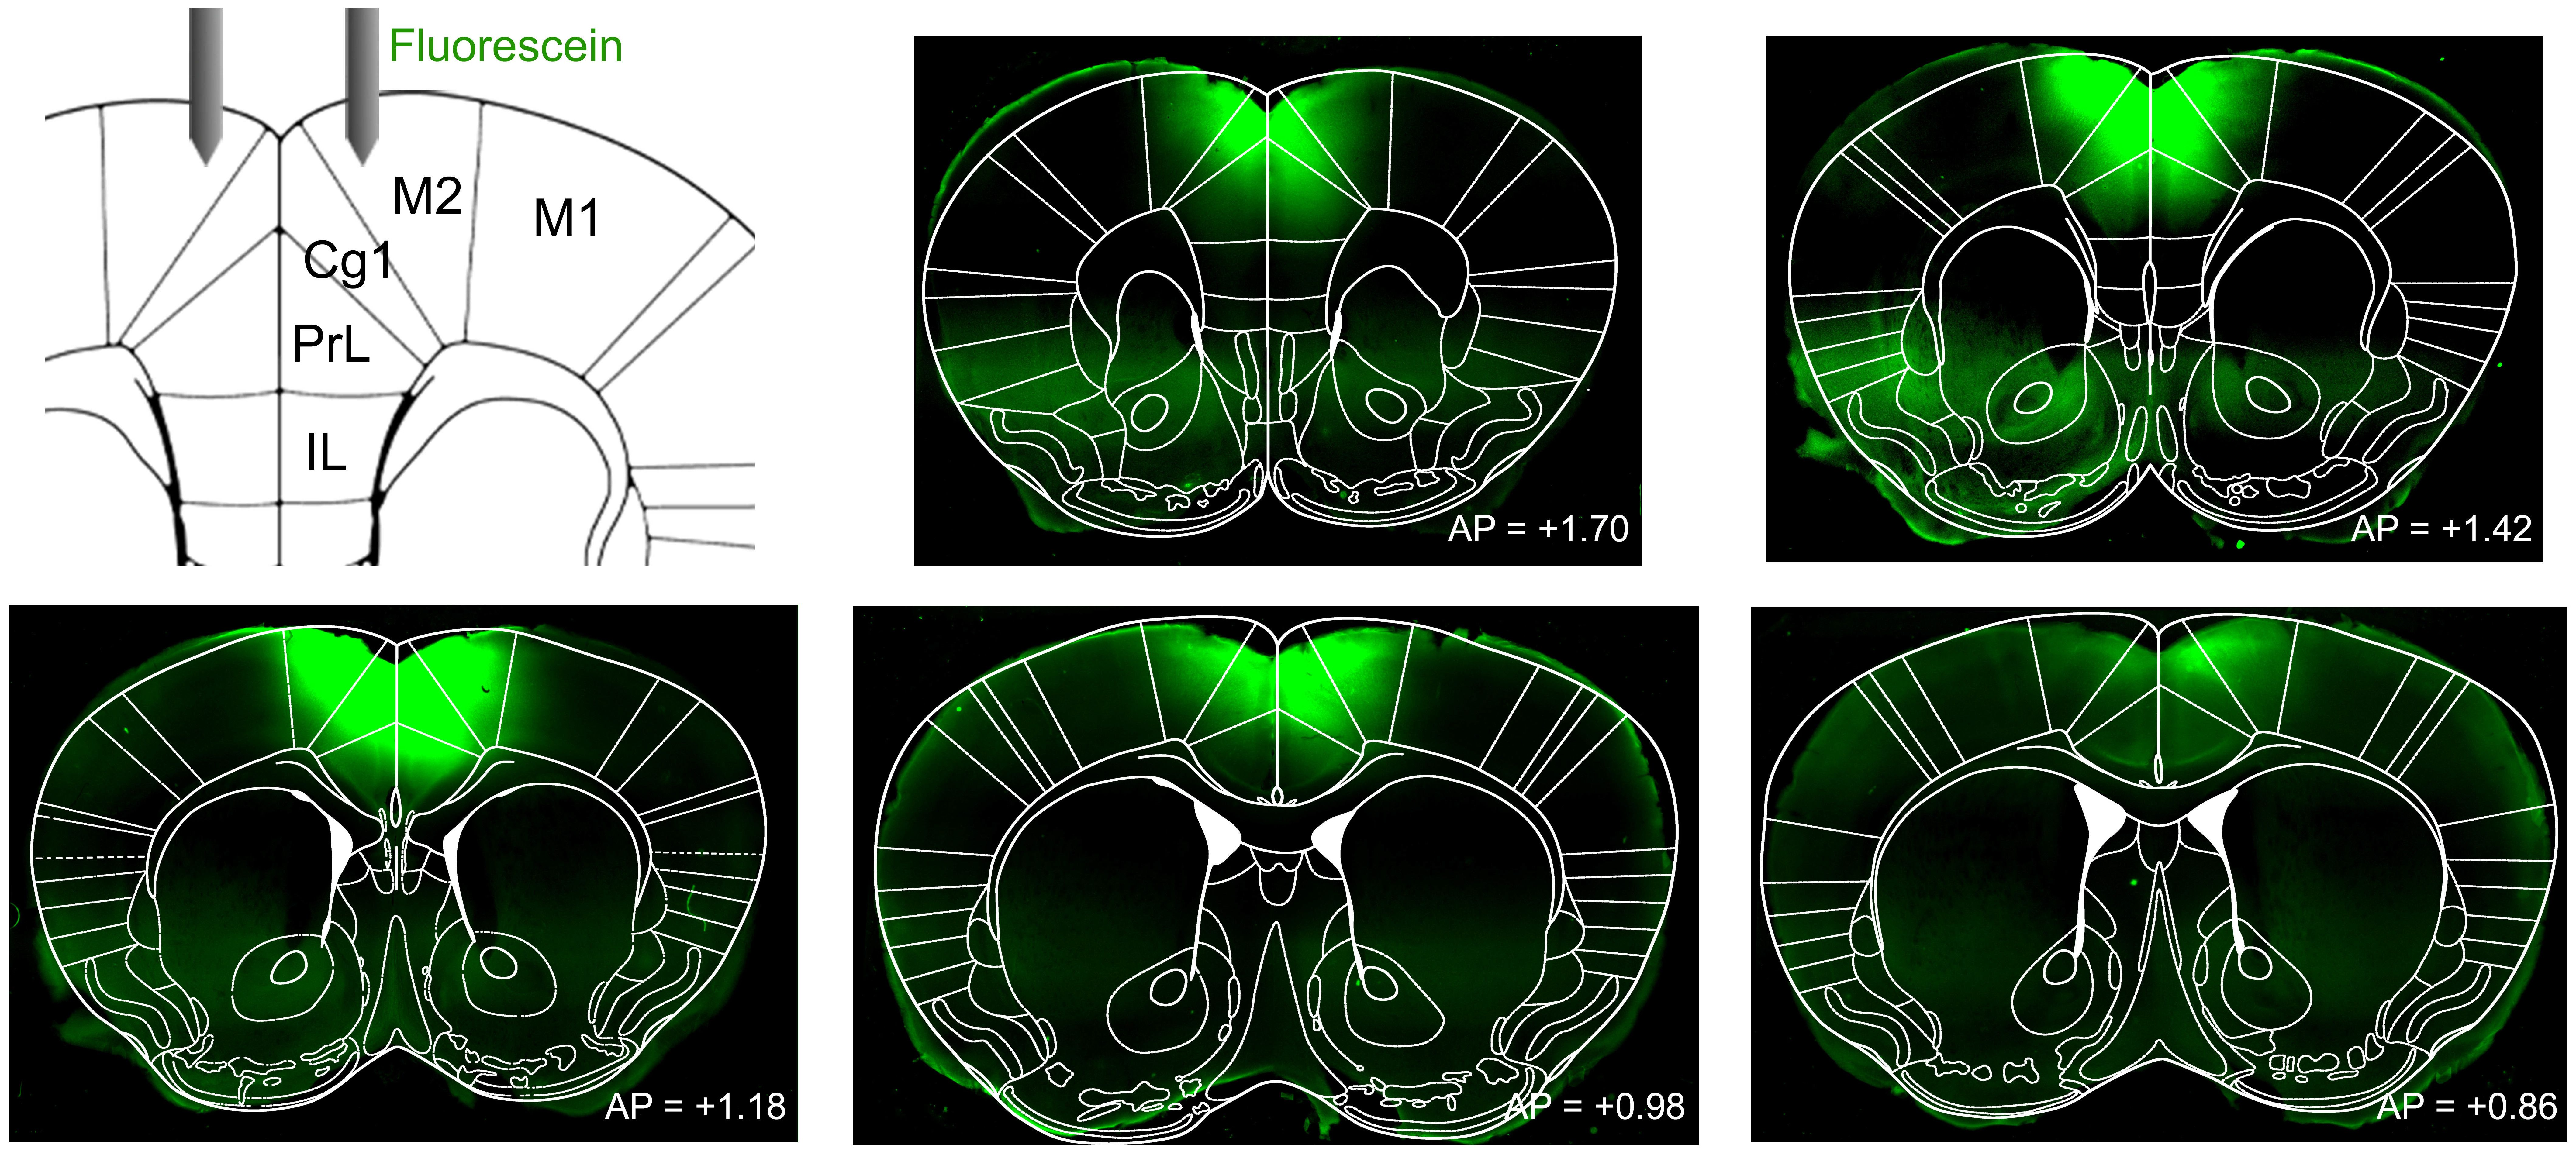
\includegraphics[width=\textwidth]{Figures/Chapter3/NN_figS4.jpg} 
\end{center}

\caption[Approximating the spread of muscimol with fluorescein]
{Approximating the spread of muscimol during inactivation experiments by injecting low-molecular-weight fluorescein.
Fluorescein (disodium salt; MW, 412; \#S25328, Fisher Scientific) was injected bilaterally into M2, at the same concentration and volume used for muscimol (5 mM, 46 nL per hemisphere). The animal was euthanized at about the time when behavioral testing would have occurred (1 hr after injections) via transcardial perfusion, and the brain was immediately sectioned with a vibratome. Using a wide-field fluorescence microscope, five images were taken for each brain slice and then stitched together to generate the figures. The image series was fitted to wire-frames from the Mouse Brain in Stereotaxic Coordinates (Franklin and Paxinos, 2008). These results showed a spread of $\sim$ 1 mm along the anterior-posterior axis. The fluorescein dye was largely restricted to M2 and Cg1.}

\label{fig:NN_figS4}
\end{figure}